\documentclass[t,usenames,dvipsnames]{beamer}
\usetheme{Copenhagen}
\setbeamertemplate{headline}{} % remove toc from headers
\beamertemplatenavigationsymbolsempty

\usepackage{amsmath, xcolor, tikz, pgfplots, array, bm}

\pgfplotsset{compat = newest}
\usetikzlibrary{arrows.meta, calc, decorations.pathreplacing}
\pgfplotsset{every axis/.append style = {axis lines = middle}}
\pgfplotsset{every tick label/.append style={font=\scriptsize}}
\everymath{\displaystyle}

\tikzstyle{input} = [circle, text centered, radius = 1cm, draw = black]
\tikzstyle{function} = [rectangle, text centered, minimum width = 2cm, minimum height = 1cm, draw = black]

\title{Logarithmic Functions}
\author{}
\date{}

\AtBeginSection[]
{
  \begin{frame}
    \frametitle{Objectives}
    \tableofcontents[currentsection]
  \end{frame}
}

\begin{document}

\begin{frame}
    \maketitle
\end{frame}

\section{Calculate logarithmic values}

\begin{frame}{Logarithms as Inverse Exponents}
The \alert{inverse} of the exponential function $f(x) = b^x$  is the {\color{blue}\textbf{logarithmic function}}. \newline\\ \pause

It is denoted
\[ f^{-1}(x) = \log_b x\]
\end{frame}

\begin{frame}{Special Bases}
The \alert{common logarithm} of a real number $x$ is $\log_{10}x$ and is usually written \[\log x\].     \pause

The \alert{natural logarithm} of a real number $x$ is $\log_e x$ and is usually written \[\ln x\].
\end{frame}

\begin{frame}{Graphs}
\begin{center}
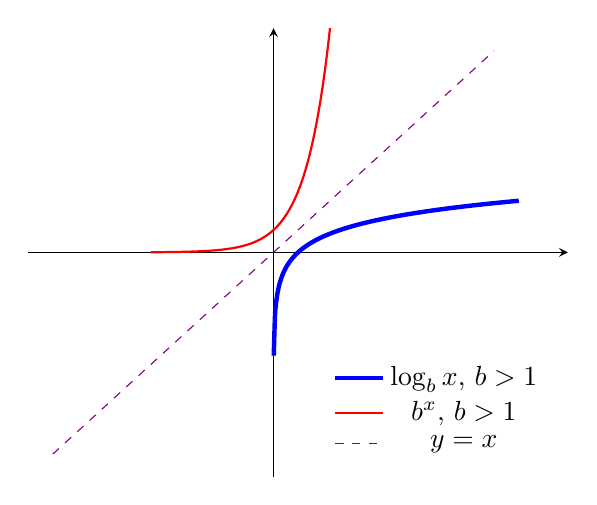
\begin{tikzpicture}
\begin{axis}[
xmin = -10, xmax = 12,
ymin = -10, ymax = 10,
ticks = none, 
legend pos = south east,
legend style={draw=none}
]
\addplot[color=blue, ultra thick, samples=200, smooth, domain=0.01:10] {ln(x)};
\addlegendentry{$\log_b x,\, b > 1$}
\addplot[color=red, thick, samples=200, smooth] {e^x};
\addlegendentry{$b^x, \, b > 1$}
\addplot[color=violet, dashed, domain=-9:9] {x};
\addlegendentry{$y=x$}
\end{axis}
\end{tikzpicture}
\end{center}    
\end{frame}

\begin{frame}{Graphs}
\begin{center}
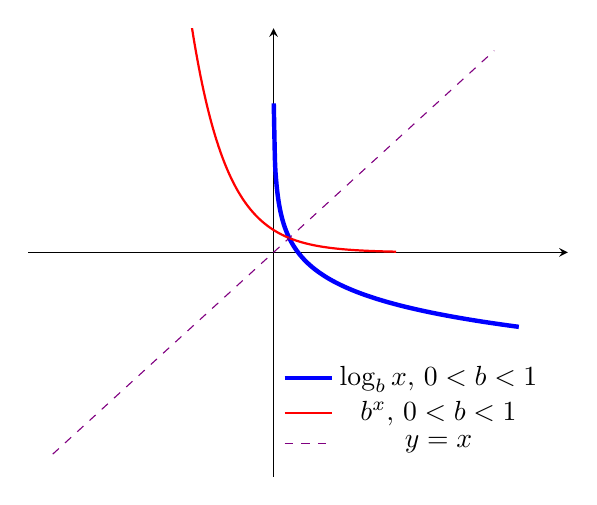
\begin{tikzpicture}
\begin{axis}[
xmin = -10, xmax = 12,
ymin = -10, ymax = 10,
ticks = none, 
legend pos = south east,
legend style={draw=none}
]
\addplot[color=blue, ultra thick, samples=200, smooth, domain=0.01:10] {ln(x)/ln(0.5)};
\addlegendentry{$\log_b x,\, 0< b < 1$}
\addplot[color=red, thick, samples=200, smooth] {0.5^x};
\addlegendentry{$b^x, \, 0 < b < 1$}
\addplot[color=violet, dashed, domain=-9:9] {x};
\addlegendentry{$y=x$}
\end{axis}
\end{tikzpicture}
\end{center}    
\end{frame}

\begin{frame}{Properties}
\begin{itemize}
    \item<+->The domain of $\log_b x$ is $(0, \infty)$ and the range is $(-\infty, \infty)$    \newline\\
    \item<+->$(1,0)$ is on the graph of $\log_b x$ and $x=0$ is a vertical asymptote.   \newline\\
    \item<+->$\log_b x$ is one-to-one (has an inverse, passes HLT), continuous, and smooth. \newline\\
    \item<+->$b^a = c$ if and only if $\log_b c = a$.   \newline\\
        \begin{itemize}
            \item<+->In other words, $\log_b c$ is the \alert{exponent} you put on $b$ to get $c$. \newline\\
        \end{itemize}
    \item<+->$\log_b b^x = x$ for all $x$ and $b^{\log_b x} = x$ for all $x >0$
\end{itemize}
\end{frame}

\begin{frame}{Properties}
For $f(x) = \log_b x \quad \text{when } b > 1$:    \newline\\
\begin{itemize}
    \item<2->$f$ is always increasing.  \newline\\
    \item<3->$\lim_{x \to 0^+} f(x) = -\infty$ and $\lim_{x \to \infty} f(x) = \infty$  \newline\\
\end{itemize}

\onslide<4->{For $f(x) = \log_b x \quad \text{when } 0 < b < 1$:} \newline\\
\begin{itemize}
    \item<5->$f$ is always decreasing. \newline\\
    \item<6->$\lim_{x \to 0^+} f(x) = \infty$ and $\lim_{x \to \infty} f(x) = -\infty$ 
\end{itemize}
\end{frame}

\begin{frame}{Example 1}
Simplify each of the following.     \newline\\
(a) \quad $\log_3 81$   
\begin{align*}
    \onslide<2->{3^{???} &= 81} \\[6pt]
    \onslide<3->{3^4 &= 81} \\[6pt]
    \onslide<4->{\log_3 81 &= 4}
\end{align*}
\end{frame}


\begin{frame}{Example 1}
(b)     \quad   $\log_2 \left(\frac{1}{8}\right)$
\begin{align*}
    \onslide<2->{2^{???} &=  \frac{1}{8}}   \\[8pt]
    \onslide<3->{2^{-3} &= \frac{1}{8}} \\[8pt]
    \onslide<4->{\log_2\left(\frac{1}{8}\right) &= -3}
\end{align*}
\end{frame}

\begin{frame}{Example 1}
(c)     \quad   $\log_{\sqrt{5}} 25$
\begin{align*}
    \onslide<2->{\left(\sqrt{5}\right)^{???} &=  25}   \\[8pt]
    \onslide<3->{\left(\sqrt{5}\right)^4 &= 25} \\[8pt]
    \onslide<4->{\log_{\sqrt{5}} 25 &= 4}
\end{align*}
\end{frame}

\begin{frame}{Example 1}
(d) \quad   $\ln \left(\sqrt[3]{e^2}\right)$  \onslide<2->{$=\ln e^{2/3}$} \onslide<3->{$=\log_{\color{red}e} e^{2/3}$}   
\begin{align*}
    \onslide<4->{{\color{red}e}^{{???}} &= e^{2/3}} \\[6pt]
    \onslide<5->{{\color{red}e}^{2/3} &= e^{2/3}}   \\[6pt]
    \onslide<6->{\ln\left(\sqrt[3]{e^2}\right) &= \frac{2}{3}}
\end{align*}
\end{frame}

\begin{frame}{Example 1}
(e) \quad $\log 0.001$  \onslide<2->{$= \log_{10} 0.001$} \onslide<3->{$=\log_{10} 10^{-3}$}
\begin{align*}
    \onslide<4->{10^{???} &= 10^{-3}} \\[6pt]
    \onslide<5->{10^{-3} &= 10^{-3}} \\[6pt]
    \onslide<6->{\log 0.001 &= -3}
\end{align*}
\end{frame}

\begin{frame}{Example 1}
(f) \quad $2^{\log_2 8}$
\begin{align*}
    \onslide<2->{\log_2 8 &= ???} \\[6pt]
    \onslide<3->{2^{???} &= 8} \\[6pt]
    \onslide<4->{2^3 = 8} \\[6pt]
    \onslide<5->{\log_2 8 &= 3} \\[6pt]
    \onslide<6->{2^{\color{red}\log_2 8} &= 2^{\color{red}3}} \\[6pt]
    \onslide<7->{&= 8}
\end{align*}
\end{frame}

\begin{frame}{Example 1}
(g) \quad $117^{-\log_{117} 6}$
\begin{align*}
    \onslide<2->{117^{-\log_{117} 6} &= \frac{1}{\color{red}117^{\log_{117} 6}}} \\[15pt]
    \onslide<3->{&= \frac{1}{6}}
\end{align*}
\end{frame}

\section{Find the domain of logarithmic functions}

\begin{frame}{Domains of Logarithmic Functions}
Up until now, the only domain restrictions we have had have been    \newline\\
\begin{itemize}
    \item Denominator can't = 0
    \item Can't take even root of a negative number
\end{itemize}
\pause

For logarithms: 

\[\log_b \, (\text{positive value}) \]    \smallskip    \pause

\[\log_b \, \big(>0\big) \]
\end{frame}

\begin{frame}{Example 2}
Find the domain of each. Write your answer in interval notation.    \newline\\
(a) \quad   $f(x) = 2\log(3-x) - 1$
\begin{align*}
    \onslide<2->{3-x &> 0} \\[6pt]
    \onslide<3->{x &< 3}
\end{align*}
\onslide<4->{\[ (-\infty, 3) \]}
\end{frame}

\begin{frame}{Example 2}
(b) \quad $g(x) = -\tfrac{2}{3}\log_8\left(x^2 + 6x - 7\right)$
\begin{align*}
    \onslide<2->{x^2 + 6x - 7 &> 0} \\[6pt]
    \onslide<3->{x^2 + 6x - 7 &= 0} \\[6pt]
    \onslide<4->{x &= -7, \, 1} \\
\end{align*}
\begin{center}
\onslide<5->{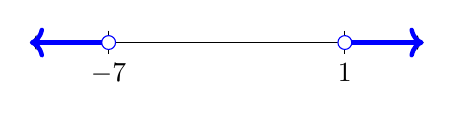
\begin{tikzpicture}
\draw[<->] (-2.5,0) -- (2.5,0);
\draw (-1.5,0.15) -- (-1.5,-0.15) node [below] {$-7$};
\draw (1.5,0.15) -- (1.5,-0.15) node [below] {$1$};
\onslide<6->{\draw[color=blue, fill=white] (-1.5,0) circle [radius=2.5pt];
\draw[color=blue, fill=white] (1.5,0) circle [radius=2.5pt];}
\onslide<7->{\draw[->, color=blue, ultra thick, shorten <= 2.5pt] (-1.5,0) -- (-2.5,0);
\draw[->, color=blue, ultra thick, shorten <= 2.5pt] (1.5,0) -- (2.5,0);}
\end{tikzpicture}}
\end{center}
\onslide<8->{\[(-\infty, -7) \cup (1, \infty)\]}
\end{frame}

\begin{frame}{Example 2}
(c) \quad $h(x) = \ln\left(\frac{x}{x-1}\right)$    
\onslide<2->{\[\frac{x}{x-1} > 0\]}
\onslide<3->{Critical values: $x = 0$ and $x = 1$}  \newline\\
\begin{center}
\onslide<4->{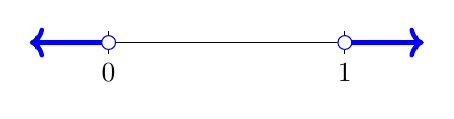
\begin{tikzpicture}
\draw[<->] (-2.5,0) -- (2.5,0);
\draw (-1.5,0.15) -- (-1.5,-0.15) node [below] {$0$};
\draw (1.5,0.15) -- (1.5,-0.15) node [below] {$1$};
\onslide<5->{\draw[color=blue, fill=white] (-1.5,0) circle [radius=2.5pt];
\draw[color=blue, fill=white] (1.5,0) circle [radius=2.5pt];}
\onslide<6->{\draw[->, color=blue, ultra thick, shorten <= 2.5pt] (-1.5,0) -- (-2.5,0);
\draw[->, color=blue, ultra thick, shorten <= 2.5pt] (1.5,0) -- (2.5,0);}
\end{tikzpicture}}
\end{center}
\onslide<7->{\[(-\infty, 0) \cup (1, \infty)\]}
\end{frame}

\end{document}
